% Raster images that decide whether the embedded file itself can become the Slides picture
% (render.image_file): a high-resolution JPEG, a CMYK JPEG, greyscale, alpha and palette PNGs,
% and the cases that must stay a render of the page (turned, mirrored, clipped, faded, labelled).
% Images are generated by make_images.py into img/.
\documentclass{beamer}
\usepackage{tikz}
\usepackage{graphicx}
\graphicspath{{img/}}
\title{Raster Image Routes}
\author{Tester}
\date{}
\beamertemplatenavigationsymbolsempty

\begin{document}

\begin{frame}{A high-resolution photo}
  \centering
  
\includegraphics[width=0.45\textwidth]{photo_big.jpg}
\end{frame}

\begin{frame}{CMYK and greyscale}
  \centering
  
\includegraphics[width=0.38\textwidth]{photo_cmyk.jpg}
  \hspace{0.06\textwidth}
  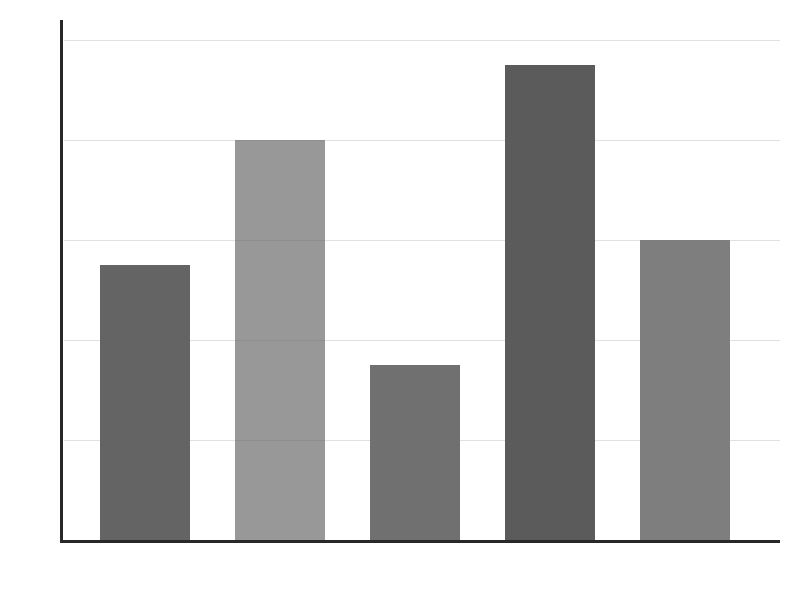
\includegraphics[width=0.38\textwidth]{plot_gray.png}
\end{frame}

\begin{frame}{Alpha and palette}
  \centering
  
\includegraphics[width=0.34\textwidth]{logo.png}
  \hspace{0.1\textwidth}
  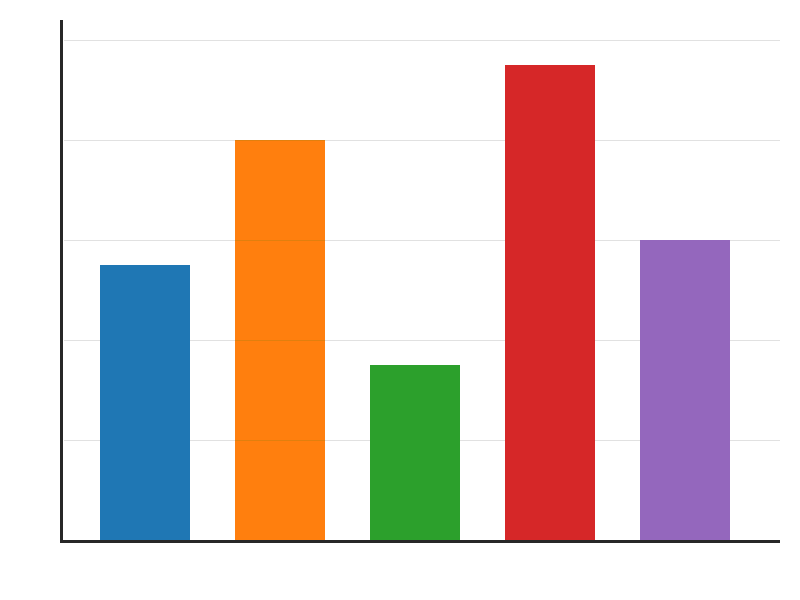
\includegraphics[width=0.38\textwidth]{plot_indexed.png}
\end{frame}

\begin{frame}{Turned and mirrored}
  \centering
  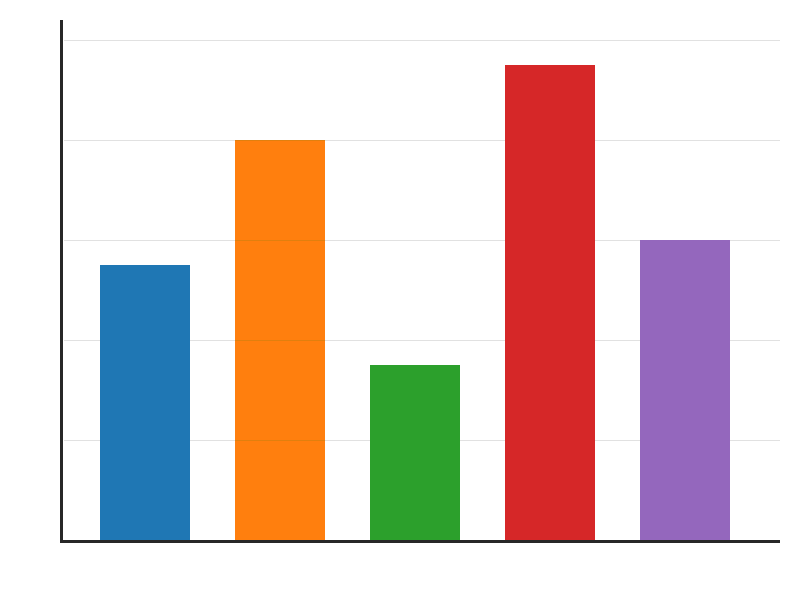
\includegraphics[angle=30, width=0.28\textwidth]{plot.png}
  \hspace{0.12\textwidth}
  \reflectbox{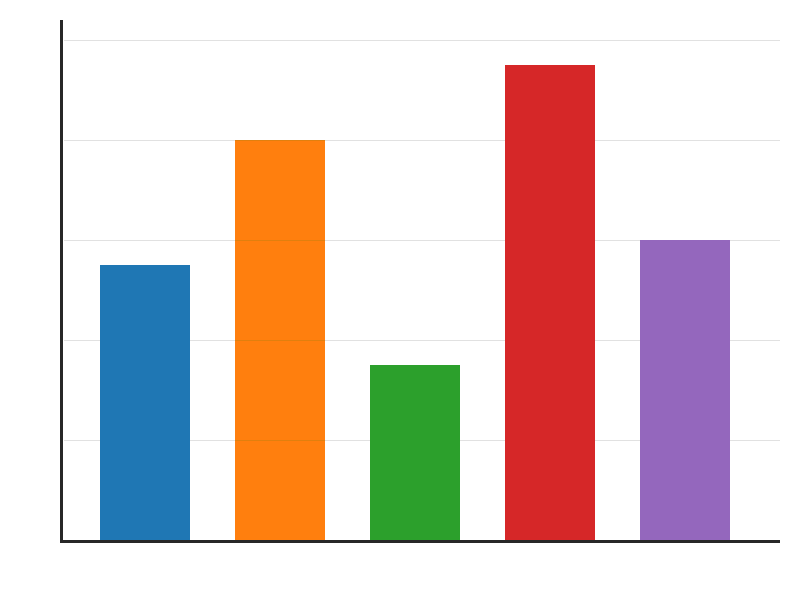
\includegraphics[width=0.3\textwidth]{plot.png}}
\end{frame}

\begin{frame}{Cut out and faded}
  \centering
  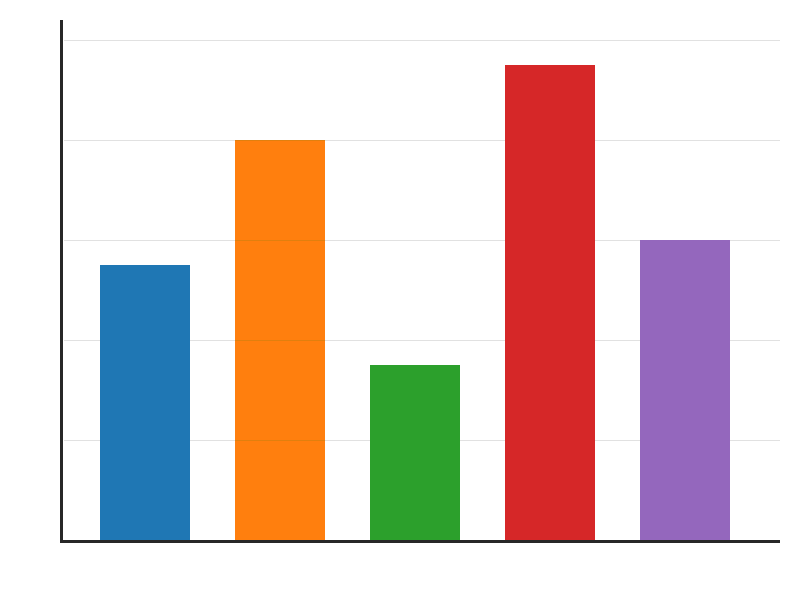
\includegraphics[trim=120 90 120 90, clip, width=0.3\textwidth]{plot.png}
  \hspace{0.1\textwidth}
  \begin{tikzpicture}
    \node[opacity=0.4, inner sep=0] {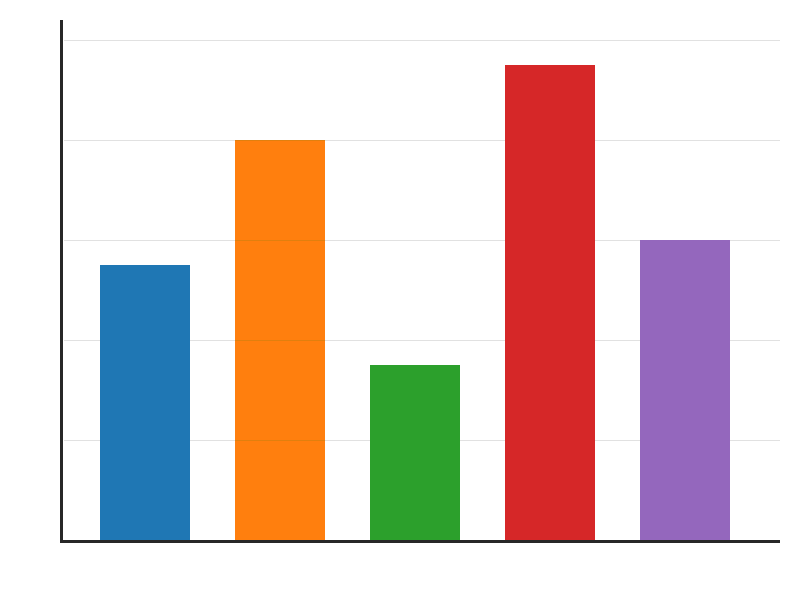
\includegraphics[width=0.3\textwidth]{plot.png}};
  \end{tikzpicture}
\end{frame}

\begin{frame}{A photo with a label}
  \centering
  
\includegraphics[width=0.45\textwidth]{photo.jpg}

  \small Fig.\ 2
\end{frame}

\end{document}
